\section{实验内容}

\textbf{实验背景}:本次实验用了 Part 1 与 Part 2 的实验背景和实验环境,在读入 WAVE 文件以及播放音频的基础上增加更多音乐播放器的功能。\\

\textbf{实验前置知识}:本次实验需要使用 C 语言来编写文件读取函数,并利用虚拟机交叉编译代码后,在开发平台上运行。因此需要提前掌握一定的 C 语言基础。同时,因为实验涉及到处理音频信号,还需要了解 Linux ALSA 音频框架。最后需要掌握 GUI 开发相关的知识。\\

\textbf{实验目标}:实现以下功能

\begin{enumerate}
    \item 调节上一曲和下一曲
    \item 实现其他格式的音乐播放,如 mp3 等
    \item 多种倍速播放(0.5,1.0,1.5,2.0 倍速)
    \item 快进快退(快进 10s,快退 10s)
    \item GUI 界面
\end{enumerate}

\section{实验部署}

程序的测试是在运行 32 位的 Debian 11 虚拟机的 Windows 主机上进行。Debian 中需要装测试以及交叉编译的依赖,可以通过运行 \code{setup.sh} 安装依赖。我们没有使用提供的交叉编译链。\\

开发板上需要将 STM32MP157 芯片启动拨码设为 EMMC 启动方式,即 101 状态,并插好电源开机。\\

开发板与主机可以直接通过以太网线链接,或通过以太网线链接到路由器。连到路由器的优点是可以通过外网访问,让所有组员可以在线上合作。开发板与主机之间的文件拷贝以及命令执行通过 Ubuntu 自带的 SCP 以及 SSH(没有使用 XShell 或 Xftp)。若开放给公网建议在开发板上设置公钥认证。

\newpage

\section{实验过程}

\subsection{源代码}

\begin{itemize}
    \item \code{audioplayer.c}:在 Part 2 实现的函数中做了以下的改善:
    \begin{itemize}
        \item \code{ap_open}:Part 2 已经实现了读入 WAVE 文件,但由于 Part 3 要求支持播放多种音频文件格式,先使用 FFmpeg 将音频文件转换成 WAVE 文件后再读入到 \code{AudioPlayer} 结构体中的 \code{data} 数组。由于需要实现调节倍速,再次使用 FFmpeg 将 WAVE 文件加速或减速存在 \code{speed_buffers} 中。此函数执行完毕后内存中会有原始音频文件的四个不同速度的版本。
        \item \code{ap_play_}:此函数是 \code{ap_play} 在新线程中调用的函数,负责调用 ALSA 库进行音频的播放。它依然按块为单位播放音频,而每块中的帧数由 \code{AP_FRAMES_PER_CHUNK} 定义。目前播放的一块的第一个字节的索引由 \code{AudioPlayer} 结构体中的 \code{at_byte} 变量记录。每块播放结束后在播放下一块前需要考虑以下三个情况:
        \begin{itemize}
            \item 倍速调节:更具倍速计算应该播放的下一个块。比如如果在 $1\times$ 倍速在播放第 12 块,则在 $0.5\times,1.5\times,2.0\times$ 倍速下一个块分别为 $24, 8, 6$。
            \item 进度调节:若用户快进或快退,则下一个块就是用户给定的时间戳对应的块。
            \item 以上两个情况都没发生,则将 \code{at_byte} 加一个块的字节个数并继续播放。
        \end{itemize}
        此外为了实现新的功能也编写了新的函数:
        \item \code{ap_get_timestamp}、\code{ap_set_timestamp}:获取以及设置时间戳。由于 \code{ap_play_} 在另一个线程也在设置时间戳所以需要用锁避免并发产生的问题。
        \item \code{ap_get_speed}、\code{ap_set_speed}:获取以及设置倍速。如果倍速不是 $0.5\times,1.5\times,2.0\times$ 之一,则默认设为 $1.0\times$。
        \item \code{ap_file_contains_audio}:使用 \code{ffprobe} 探测一个文件中是否存在音频数据。
        \item \code{ap_scan_dir}:找出当前目录下所有音频文件并存在 \code{audio_filenames} 中,为调节上一曲和下一曲以及 GUI 的播放列表调用。
    \end{itemize}
    \item \code{audioplayer_gui.c}:为 \code{audioplayer} 实现了 GUI
    \begin{itemize}
        \item \code{audioplayer_gui} 函数是入口函数,负创建 \code{AudioPlayer} 对象以及 GTK 应用
        \item \code{activate} 函数负责初始化界面,创建各个部件,连接部件的回调函数
        \item \code{timeout} 函数每 10 毫秒调用一次,负责更新界面,比如播放进度、播放进度条等等
        \item 其余函数都在某个部件的某个事件触发后被调用
    \end{itemize}
\end{itemize}

\subsection{编译与运行}

测试编译(\code{make debug})以及交叉编译(\code{make xc})的命令都在 \code{Makefile} 中定义。使用的交叉编译器是 \code{arm-linux-gnueabihf-gcc}。需要链接三个库:用于播放声音的 \code{libasound} 、用于实现多线程的 \code{pthread}、以及图形界面库 \code{gtk3}。为了避免没必要的编译步骤,\code{make copy-libs} 利用在开发板上已有的动态二进制库,将其拷贝到主机开发环境中。

将可执行文件拷贝到开发板上用 \code{make scp},需要保证 \code{SXX_KEY}、\code{SXX_PORT}、\code{SXX_HOST} 变量与实际情况一致。在主机上和在开发板上正常运行程序的命令分别为 \code{make drun} 和 \code{make xrun}。

\newpage

\section{实验结果}

预期完成的功能都成功地实现了。以下是 GUI 功能介绍:

\begin{figure}[h!]
    \centering
    \begin{tikzpicture}
        \node[anchor=south west,inner sep=0] at (0,0) {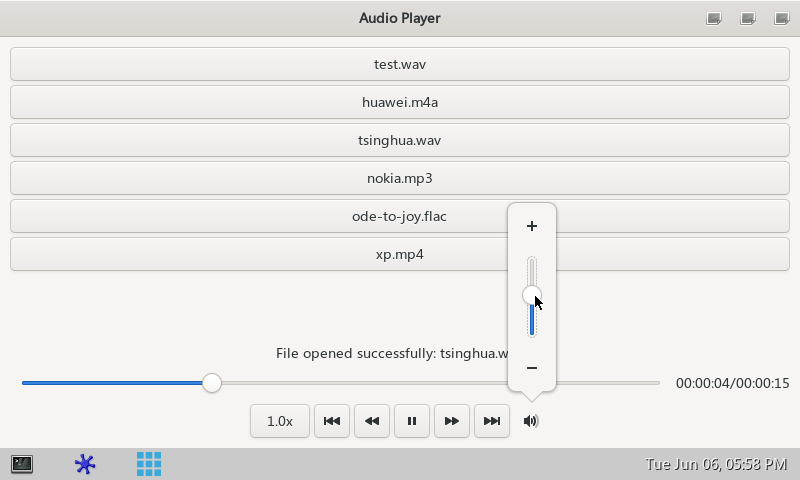
\includegraphics[width=\textwidth]{imgs/screenshot.png}};
        \node[red] at (0.2,4) {1};
        \node[red] at (4.4,2.5) {2};
        \node[red] at (8,3) {3};
        \node[red] at (10.3,3.8) {4};
        \node[red] at (15,2.5) {5};
        \node[red] at (5.8,1.8) {6};
        \node[red] at (6.9,1.8) {7};
        \node[red] at (7.7,1.8) {8};
        \node[red] at (8.5,1.8) {9};
        \node[red] at (9.3,1.8) {10};
        \node[red] at (10.1,1.8) {11};
    \end{tikzpicture}
\end{figure}

\begin{multicols}{2}
\begin{enumerate}
    \item 播放列表:列出文件夹中所有包含音频数据的文件,可以通过点击切换目前播放的音频文件
    \item 播放进度条
    \item 播放状态信息
    \item 音量调节
    \item 播放进度
    \item 倍速:点击后在 $1.0\times, 1.5\times, 2.0\times, 0.5\times$ 倍速之间切换
    \item 调节上一曲
    \item 快退十秒
    \item 播放/暂停
    \item 快进十秒
    \item 调节下一曲
\end{enumerate}
\end{multicols}

\newpage

\section{实验心得}

Part 3 实验过程中遇到的问题及其解决方法如下:

\begin{itemize}
    \item 虚拟机与交叉编译:在交叉编译调用 GTK 库的过程中遇到了问题,因为安装的 GTK 头文件中有假设浮点数必须为 64 位的断言。为了避免做更多的交叉编译配置,直接查找了满足 glibc 版本要求并且是 32 位的操作系统,很快找到了满足要求的 Debian 11。
    \item FFmpeg 格式转换:使用 FFmpeg 将不同音频格式转换成 WAVE 格式后,它似乎不符合 WAVE 文件的格式。查看文件的二进制信息后发现 FFmpeg 在 WAVE 头的 data chunk 后加入了额外的编码信息。使用 \code{-fflags +bitexact} 参数删掉了这些额外信息,产生了符合标准的 WAVE 文件。
    \item GUI:由于 QT 需要使用 \code{qmake},并且使用 C++ 语言,而已有的代码是用 C 写的,并且开发板已经支持 GTK,因此选择使用 GTK。我们从来没有用过 GTK 做图形界面,但是对于这个比较简单的界面上手较快。在开发过程中需要注意的事项包括 GTK 函数只能在主线程中调用,因此我们需要改变我们的编程思维,特别是如何处理多线程的问题。
    \item 倍速调节:调节倍速功能可能是最花费时间的功能。最初的实现方法是简单地调节 ALSA 的采样率。虽然这的确加快了播放速度,但是也导致了音色失真。参考了更多资料 \footnote{\url{https://en.wikipedia.org/wiki/Audio_time_stretching_and_pitch_scaling}}\footnote{\url{https://dsp.stackexchange.com/questions/31850/slow-down-music-playing-while-maintaining-frequency}} 后发现在保持音色不变的前提下改变播放速度需要用到比较复杂的算法。试图使用 \href{https://github.com/dbry/audio-stretch}{\code{audio-stretch}} 库虽然达到了以上的目标,但是实时的音频倍速处理将播放的音频比较卡顿。这个问题可能可以使用多线程缓冲处理过的数据来实现,但是实现的复杂度与出现代码问题的可能性都会增加很多。因此最后的解决方案就是在打开音频文件处理后再进行播放。这个方法的两个弊端是处理时间较长会降低用户体验,并且若音频文件太大会有内存不足的问题。由于 FFmpeg 有 \code{atempo} 过滤器,所以就没有用 \code{audio-stretch} 而是直接用 FFmpeg 实现倍速功能。
\end{itemize}

从此大作业的三个部分,所有组员不仅学会了如何为嵌入式系统开发软件,而且也了解了如何使用多种框架,训练了解决问题的能力,以及提高了作为软件工程师必备的技能。